\documentclass[12pt, titlepage]{article}
\usepackage{xcolor} % for different colour comments

%% Comments
\newif\ifcomments\commentstrue

\ifcomments
\newcommand{\authornote}[3]{\textcolor{#1}{[#3 ---#2]}}
\newcommand{\todo}[1]{\textcolor{red}{[TODO: #1]}}
\else
\newcommand{\authornote}[3]{}
\newcommand{\todo}[1]{}
\fi

\newcommand{\wss}[1]{\authornote{magenta}{SS}{#1}}
\newcommand{\ds}[1]{\authornote{blue}{DS}{#1}}

%% Graphics
\usepackage{float}
\usepackage{caption}
\usepackage{graphicx}
\usepackage{courier}
\graphicspath{ {images/} }

\begin{document}

\title{Smart Waiter Test Report} 
\author{Meraj Patel \#1137491 \\ Pavneet Jauhal \#1149311\\ Shan Perera \#1150394}
\date{\today}
\maketitle

\tableofcontents 

\listoftables

\begin{table}[H]
\section*{Revision History}
\begin{tabular}{|c|c|}
\hline
\textbf{Date}  & \textbf{Comments} \\ \hline
March 20, 2016 & Test results added \\
\hline
\end{tabular}
\caption{Revision History Table}
\end{table}

\section{Introduction}

\section{System Testing} 
\subsection{Barcode Scanning}

\subsubsection{Purpose}
Barcode scanning tests were conducted to make sure users are able to scan a barcode with minimal attempts. Also, to check if appropriate messages are displayed according to each test case.

\subsubsection{Functional Unit Test}
As per our test plan, functional unit tests were  conducted to assess test cases. Doing so replicates real world usage.

\subsubsection{Test Results}
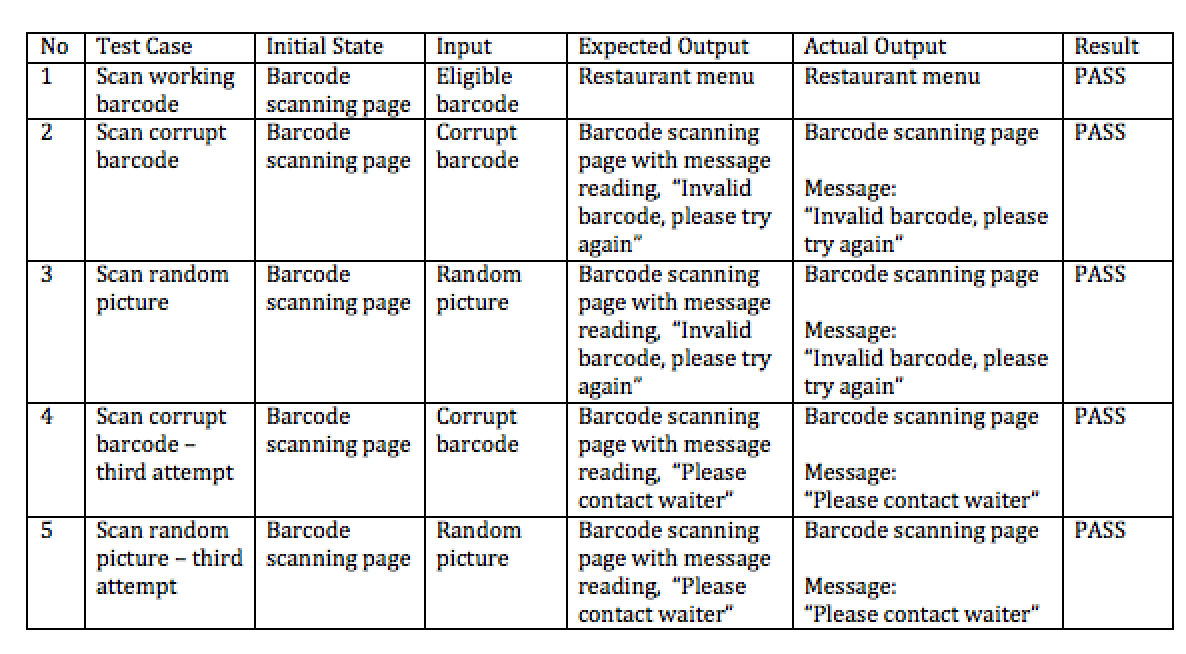
\includegraphics[width=1.2\textwidth]{barcodeTable.png}

\subsection{Accounts}
\subsubsection{Functional Dynamic Test}
As per our test plan, manual functional dynamic tests we performed to assess the following test cases. This allows the system to be exhaustively tested which will minimize or completely erase errors in real world usage.
\subsubsection{Purpose}
Account creation and login tests were performed to ensure Smart-Waiter users are able to create an account quickly while still adhering to the account constraints set by Smart-Waiter. This is also to ensure proper error checking is implemented in the applications account related modules.

\subsubsection{Test Results}
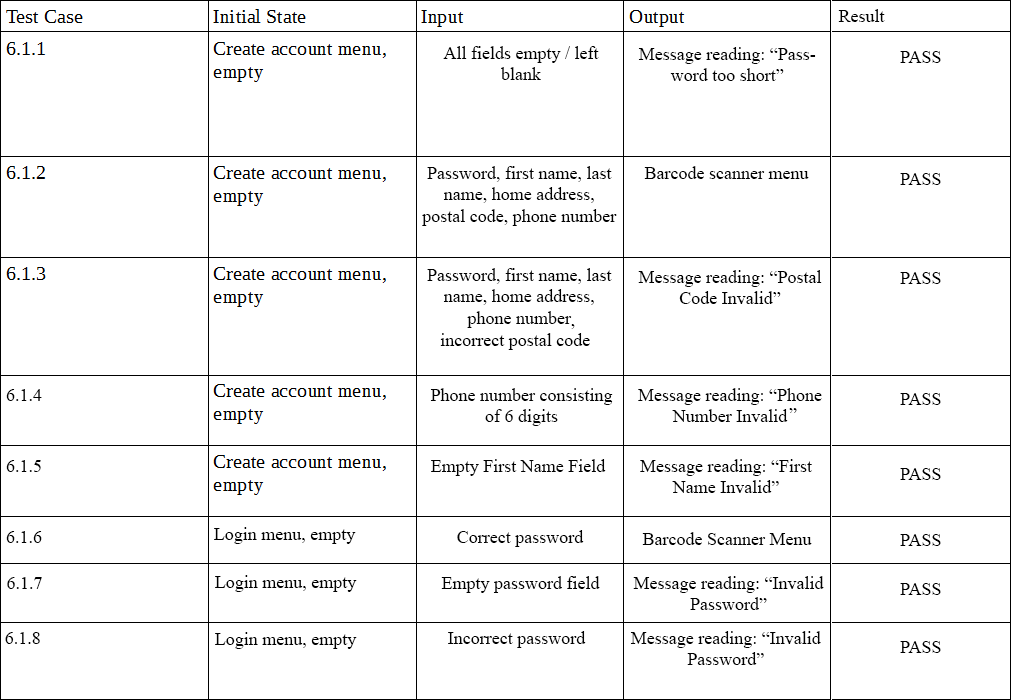
\includegraphics[width=1.2\textwidth]{accountTC.png}
\section{Usability Test}
Usability tests are conducted to assess the user's ability to complete routine tasks, and acquire their impression of the application.
\subsection{Summary}

To retrieve insightful results, participants were asked to complete a series of tasks and answer a brief questionnaire afterwards. 
\\\\
The first usability test has already been conducted on February 4, 2016. A total of six participants were gathered to conduct this test. To replicate an adequate demographic, three participants chosen are experienced using android applications, while the remaining three have little to no experience. 
\\\\
The proceeding sections provide insight and results of the usability test conducted. 

\subsection{Methodology}

\subsubsection{Tasks conducted}
Participants were given a list of tasks to complete including: 
\begin{itemize}  
\item Task 1: Create and login to account
\item Task 2: Scan barcode to retrieve menu
\item Task 3: Customize and add items to cart
\item Task 4: View cart
\item Task 5: Delete item
\item Task 6: Modify item
\item Task 7: Confirm and pay for order
\end{itemize}
\subsubsection{Questionnaire}
Participants were asked to rate from 1 to 5 (1 - strongly disagree, 5 - strongly agree), provided the following statements: 
\begin{enumerate}
\item  I was able to complete the task quickly using the system
\item It was easy to learn how to use the system
\item I prefer using Smart-Waiter over ordering in a traditional sense
\item The interface of the system was pleasant
\item The system has all the functions and capabilities I expect it to have
\item Whenever I made a mistake using the system, I could recover easily and quickly
\item Overall I was happy using the system
\end{enumerate} 

\subsection{Testing Results} 

\subsubsection{Questionnaire Results}

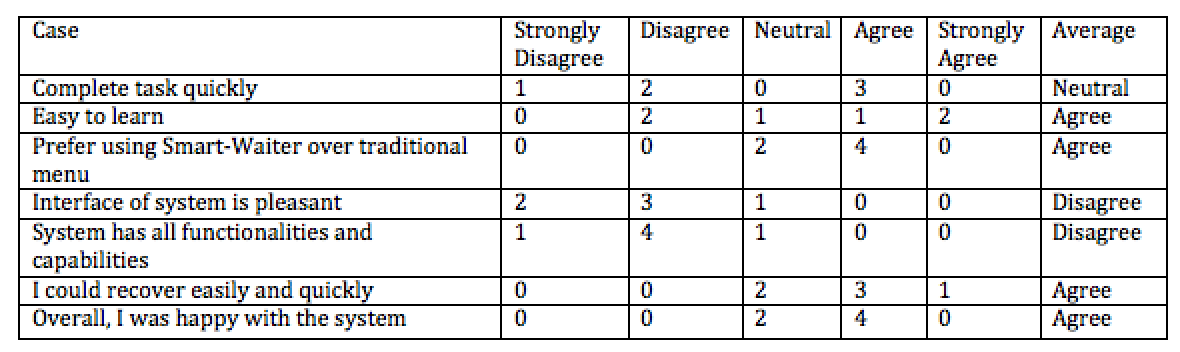
\includegraphics[width=1.2\textwidth]{usabilityResults.png}

\subsubsection{User Feedback}

After completing the usability test, we asked participants for feedback in terms of their experience. Specifically we asked for their; likes, dislikes and recommendations. 
\\\\
\textbf{Likes} 
\begin{itemize}
\item Convenient for ordering take out at restaurant  
\item Ability to customize items and send special instructions
\item Ease of use (according to experienced android application users)
\end{itemize}
\textbf{Dislikes}
\begin{itemize}
\item Look of GUI
\item Unable to modify account settings
\item Unable to save receipt 
\end{itemize}
\textbf{Recommendations}  
\begin{itemize}
\item Add settings page
\item Offer ability to email receipt
\end{itemize}
\subsection{Conclusion}
Conducting this usability test definitely helps our team in terms of adjusting requirements to meet user recommendations. Specifically the following changes will be implemented: 
\begin{itemize}
\item Create settings page
\item Improve GUI
\item Allow users to view order history
\end{itemize}
After implementation of these additions, a second usability test will be conducted. New participants will be gathered in order to provide unbiased results. 
\end{document}